
\chapter{On the relationship between Arctic fall season precipitation and minimum sea ice extent}
\label{chap:fall_prec}

This chapter is to be submitted to \textit{Journal of Geophysical Research - Atmospheres} as

\hangbibentry{Hamman_2016f}

\section*{Abstract}

Over the past three decades, the Arctic has experienced large declines in summer sea ice cover, permafrost extent and spring snow cover, as well as increases in fall precipitation.
This study explores the relationship between declining Arctic sea ice extent and fall season precipitation across the high-latitude Arctic land masses.
The first part of this paper presents the observed relationship between sea ice extent and fall precipitation.
Using satellite estimates of sea ice extent and precipitation data based on in-situ observations, we show that fall season precipitation across the Pan Arctic drainage basin is broadly negatively correlated with summer sea ice extent.
We hypothesize that the observed correlation between sea ice extent and high-latitude precipitation is related to anomalous patterns in ocean evaporation and sea ice extent in the fall.
To better understand the physical mechanisms driving the observed changes in the Arctic climate system and the sensitivity of the Arctic climate system to declining sea ice, we have used the fully-coupled Regional Arctic System Model (RASM) to simulate three distinct sea ice climates.
The first climate represents normal sea ice extent, while the second and third represent reduced summer sea ice extent.
The second part of this paper analyzes these three RASM simulations, in conjunction with our observation-based analysis, to understand the relationship between poleward moisture transport, sea ice extent, evaporation from the Arctic Ocean, and precipitation.
We will present the RASM-simulated Arctic water budget and demonstrate the role of sea ice extent in driving fall precipitation anomalies.
Finally, we use the Self-Organizing Map (SOM) machine learning technique to identify characteristic patterns of ocean evaporation and sea ice extent that contribute to anomalies in fall season precipitation.

\section{Introduction}
\label{sec:intro_ch5}

During the last thirty-five years, the Arctic region has experienced unprecedented changes in key cryospheric processes.
Rapid declines in sea ice cover have been accompanied by reductions in permafrost extent and spring snow cover, as well as increases in seasonal precipitation and winter snow accumulations \citep{Kohler_2006,Callaghan_2011,Bulygina_2009,Screen_2012}.
These combined changes have had a marked impact on the regional and global climate systems.
Driving much of these changes has been a regional warming trend that is nearly twice as large as the global mean \citep{Serreze_2006c,Screen_2010}.
This disparity in temperature increases is often referred to as Arctic Amplification and is largely explained by the ice-albedo feedback \citep{Curry_1995}.
While this is likely the primary mechanism that leads to rapid warming in the Arctic, other, secondary feedback processes are also at play.
One such feedback process relates the state and fluxes of the Arctic Ocean (sea surface temperatures or SSTs, sea ice cover, evaporation) to precipitation over land, which modulates winter snow cover and permafrost health.

Observational evidence of an amplified hydrologic cycle \citep{Stocker_2005} has been found in the form of increasing precipitation \citep{Rawlins_2006}, runoff \citep{Peterson_2002}, and winter snow accumulations \citep{Kohler_2006,Bulygina_2009,Screen_2012}.
While global average precipitation is expected to increase following a response to warming via the Clausius-Clapeyron relationship \citep[e.g.][]{Held_2006,Stephens_2008,Byrne_2015}, precipitation increases in the Arctic are expected to exceed the global average \citep{Stocker_2005}.
Analysis of the collection of Earth system models (ESMs) in the Coupled Model Intercomparison Project Phase 5 \citep[CMIP5;][]{Taylor_2012} by \citet{Bintanja_2014} indicates that annual precipitation changes in the Arctic may exceed 50\%, with the largest relative increases in the early winter (October-January) over the Arctic Ocean when precipitation has typically been low.
\citet{Bintanja_2014} also identify that most of these changes are due to precipitation sourced from enhanced local evaporation related to retreating sea ice.
This somewhat contradicts previous work that suggested increased poleward moisture transport as the main driver of Arctic precipitation increases \citep{Bengtsson_2011}.
Combined with the large intermodel spread of precipitation changes in their study, this contradiction brings into question the sensitivity of the response of Arctic precipitation to reduced sea ice in modern ESMs.
ESMs, along with statistical models, tend to poorly represent the observed decline in summer sea ice extent.
This is evidenced by the intermodel spread among the 39 ESMs analyzed by \citet{Bintanja_2014}.
In their study, changes in sea ice extent between the beginning and end of the twenty-first century ranged between 31-66\%, while changes in precipitation varied by a factor of three to four.

Conceptually, a warmer Arctic Ocean with less sea ice will lead to increased surface evaporation and may lead to enhanced divergence of moisture onto land in the form of precipitation.
Because high-latitude land areas are predominantly below freezing in the fall, increases in precipitation during this season are expected to produce deeper snow packs.
This process would then act to insulate the underlying ground during winter and suppress cold season cooling of high-latitude permafrost \citep{Osterkamp_1999,Zhang_2005,Lawrence_2010}.
Further permafrost degradation may be attributed to earlier spring snow melt driven by regional warming and possibly by increased surface infiltration of warm meltwater \citep{Lawrence_2010}.

How the Arctic climate will respond to such large temperature and sea ice changes has been at the forefront of recent studies \citep[e.g.][]{Kazutoshi_2014,Simmonds_2014,Wegmann_2015,Vihma_2014}.
Here, we investigate the relationship between Arctic fall precipitation, ocean evaporation, and sea ice extent to better understand the terrestrial precipitation response to the ongoing sea ice decline.
Our a priori hypothesis is that the reductions in sea ice extent lead to increases in evaporation from the central portions of the Arctic Ocean and precipitation over land during the fall season.
We explore this hypothesis using three simulations spanning a range of sea ice climates from a fully-coupled regional ESM described in Section \ref{sec:data_models_ch5}.
In Section \ref{sec:results_ch5} we present our analysis of these simulations, first computing the regional freshwater budget following \citet{Serreze_2006a}, then using the Self-Organizing Map (SOM) machine learning technique for dimension reduction and pattern evaluation \citep{Kohonen_1998,Hewitson_2002}.

\section{Data and Methods}
\label{sec:data_models_ch5}

\subsection{Model Simulations and Observations}
We use three simulations from the Regional Arctic System Model \citep[RASM;][]{Hamman_2016a,Roberts_2015a}.
RASM is a high-resolution, fully-coupled regional ESM that has been recently developed to improve the representation of coupled Arctic processes.
RASM is comprised of individual land \citep[see][]{Hamman_2016a}, atmosphere \citep[see][]{Cassano_2016}, ocean \citep[see][]{Roberts_2015a}, sea ice \citep[see][]{Roberts_2015a}, and runoff \citep[see][]{Hamman_2016b} components, coupled via the CESM flux coupler \citep{Craig_2012}. % BN: No space after the text in \citep[text] - latex already adds one.
In RASM, the atmosphere is forced at its lateral boundaries with the ERA-Interim Reanalysis \citep{Dee_2011} and the ocean's closed boundaries are relaxed to the climatology from \citet{Steele_2001}.
It is important to note that spectral nudging is applied to temperature and winds in RASM above 500 hPa.
From a practical perspective, the impact of this nudging means that the synoptic scale circulation patterns in all three RASM simulations closely match those of ERA-Interim \citep{Glisan_2013}.
The land, atmosphere, and runoff components in RASM are applied on a 50 km near equal area polar stereographic grid while the ocean and sea ice are applied on a 1/12$^{\circ}$ rotated pole mesh.

Each of the three RASM simulations used here were run from September 1, 1979 through December 31, 2014, although our analysis begins after a 5-year spinnup to allow for the stabilization of the ocean and sea ice components under coupled forcings.
\citet{Hamman_2016b} provide a complete description of the configuration of RASM for the baseline $RASM_{CONTROL}$ simulation.
Two sensitivity simulations, $RASM_{RSI}$ and $RASM_{RSH}$, representing intermediate and high reductions in sea ice extent are also analyzed.
The configuration of these simulations is identical to $RASM_{CONTROL}$ except in the parameterization of sea ice albedos, which is summarized in Table \ref{table:sims}.
Sea ice albedo is reduced in both simulations to promote accelerated spring sea ice melt and reduced sea ice extent in the spring and summer.
This method of altering the radiative properties of sea ice allows for fully-coupled, physically-consistent simulations in RASM and avoids the need for prescribed surface conditions that are not physically-realistic or that lead to inconsistencies in the coupling fields.

\begin{table}[]
    \centering
    \caption{Summary of RASM simulations used in this chapter.}
    \label{table:sims}
    \begin{tabular}{|l|p{4in}|}
    \hline
    \textbf{Dataset} & \textbf{Sea Ice / Ocean Configuration}                                                                                                         \\ \hline
    $RASM_{CONTROL}$    & Default RASM [see \citet{Hamman_2016b}]                                                                                                          \\ \hline
    $RASM_{RSI}$         & \begin{tabular}[c]{@{}l@{}}Ocean: No changes\\ Sea Ice: Snow grain diameter -0.5 std. dev. of observed.\end{tabular}                                   \\ \hline
    $RASM_{RSH}$         & \begin{tabular}[c]{@{}p{3.5in}}Ocean: No changes\\ Sea Ice: No sea ice initial condition, reduced snow grain diameter and ice/pond albedo -2.0 std. dev.
    \end{tabular} \\ \hline
    \end{tabular}
\end{table}

Observations of sea ice extent are taken from the National Snow and Ice Data Center (NSIDC) Weekly Sea Ice Extent product \citep{Brodzik_2013}.
Gridded precipitation observations between 1979 and 2014 are taken from CRU TS v.3.23 \citep{Harris_2014}.

\subsection{Self-Organizing Maps}
In Section \ref{sec:rasm_results}, we present results using the Self-Organizing Maps algorithm \citep[SOMs][]{Kohonen_1998,Hewitson_2002}, which is a technique for dimension reduction that allows for the identification of unique climatological patterns.
SOMs are a type of unsupervised machine learning, utilizing artificial neural networks to create a lower-dimensional representation of high-dimensional datasets.
They have been applied previously in studies of polar climatology to study synoptic scale atmospheric circulation \citep[e.g.][]{Cassano_2007}, extreme weather events \citep[e.g.][]{Cassano_2015,Glisan_2016}, and coupled ocean-atmosphere processes \citep[e.g.][]{DuVivier_2016}.

In our analysis, we trained a 2x4 SOM, using standardized ocean evaporation anomalies north of 55$^{\circ}$ N from the three RASM simulations described in Section \ref{sec:data_models_ch5} for individual fall months (August-October) between 1985 and 2014.
In total, the training dataset combines the three simulations, resulting in 270 months of evaporation anomalies.
By combining the three RASM simulations, we effectively increase the training dataset space and allow for the determination of changes in pattern occurrence between the simulations.
Standardized anomalies were calculated relative to the climatology for the entire analysis period.
We used an evaluation metric of Euclidean distance, a learning rate of 0.001, and a maximum number of iterations of 2000.
The shape of the 2x4 SOM was chosen to provide a sufficient number of unique patterns while maximizing the average number of samples in each pattern.
The SOM was initialized with spatially independent random fields from a standard normal distribution.
Further details on the SOM algorithm can be found in \citet{Reusch_2005} or \citet{Cassano_2015}.

\section{Results and Discussion}
\label{sec:results_ch5}
\subsection{Observational evidence}
% Motivation and establishing a connection between sea ice extent and precipitation
Our hypothesized relationship between precipitation and sea ice extent builds on the observed interannual covariation of precipitation and minimum sea ice extent across the Arctic drainage basin.
Here we define the Arctic drainage basin as the land areas draining to the ocean model within the RASM model.
Figure \ref{fig:prec_spatial_corr} shows the Spearman rank-order correlation coefficients between minimum annual sea ice extent and seasonal total precipitation between August-October from the CRU dataset at each grid point within the Arctic drainage basin.
Across most of the Siberian portion of the domain, correlations or consistently negative with values as low as -0.55.
Conversely, correlations across North America and northern Europe are predominantly near zero or positive.
Generally, a moderately consistent relationship exists between sea ice extent and precipitation, especially in the high-latitude regions of the study domain.
In the following sections, we will explore this relationship further with the goal of understanding the observed spatial patterns and driving mechanisms.

\begin{figure}
  \centering
  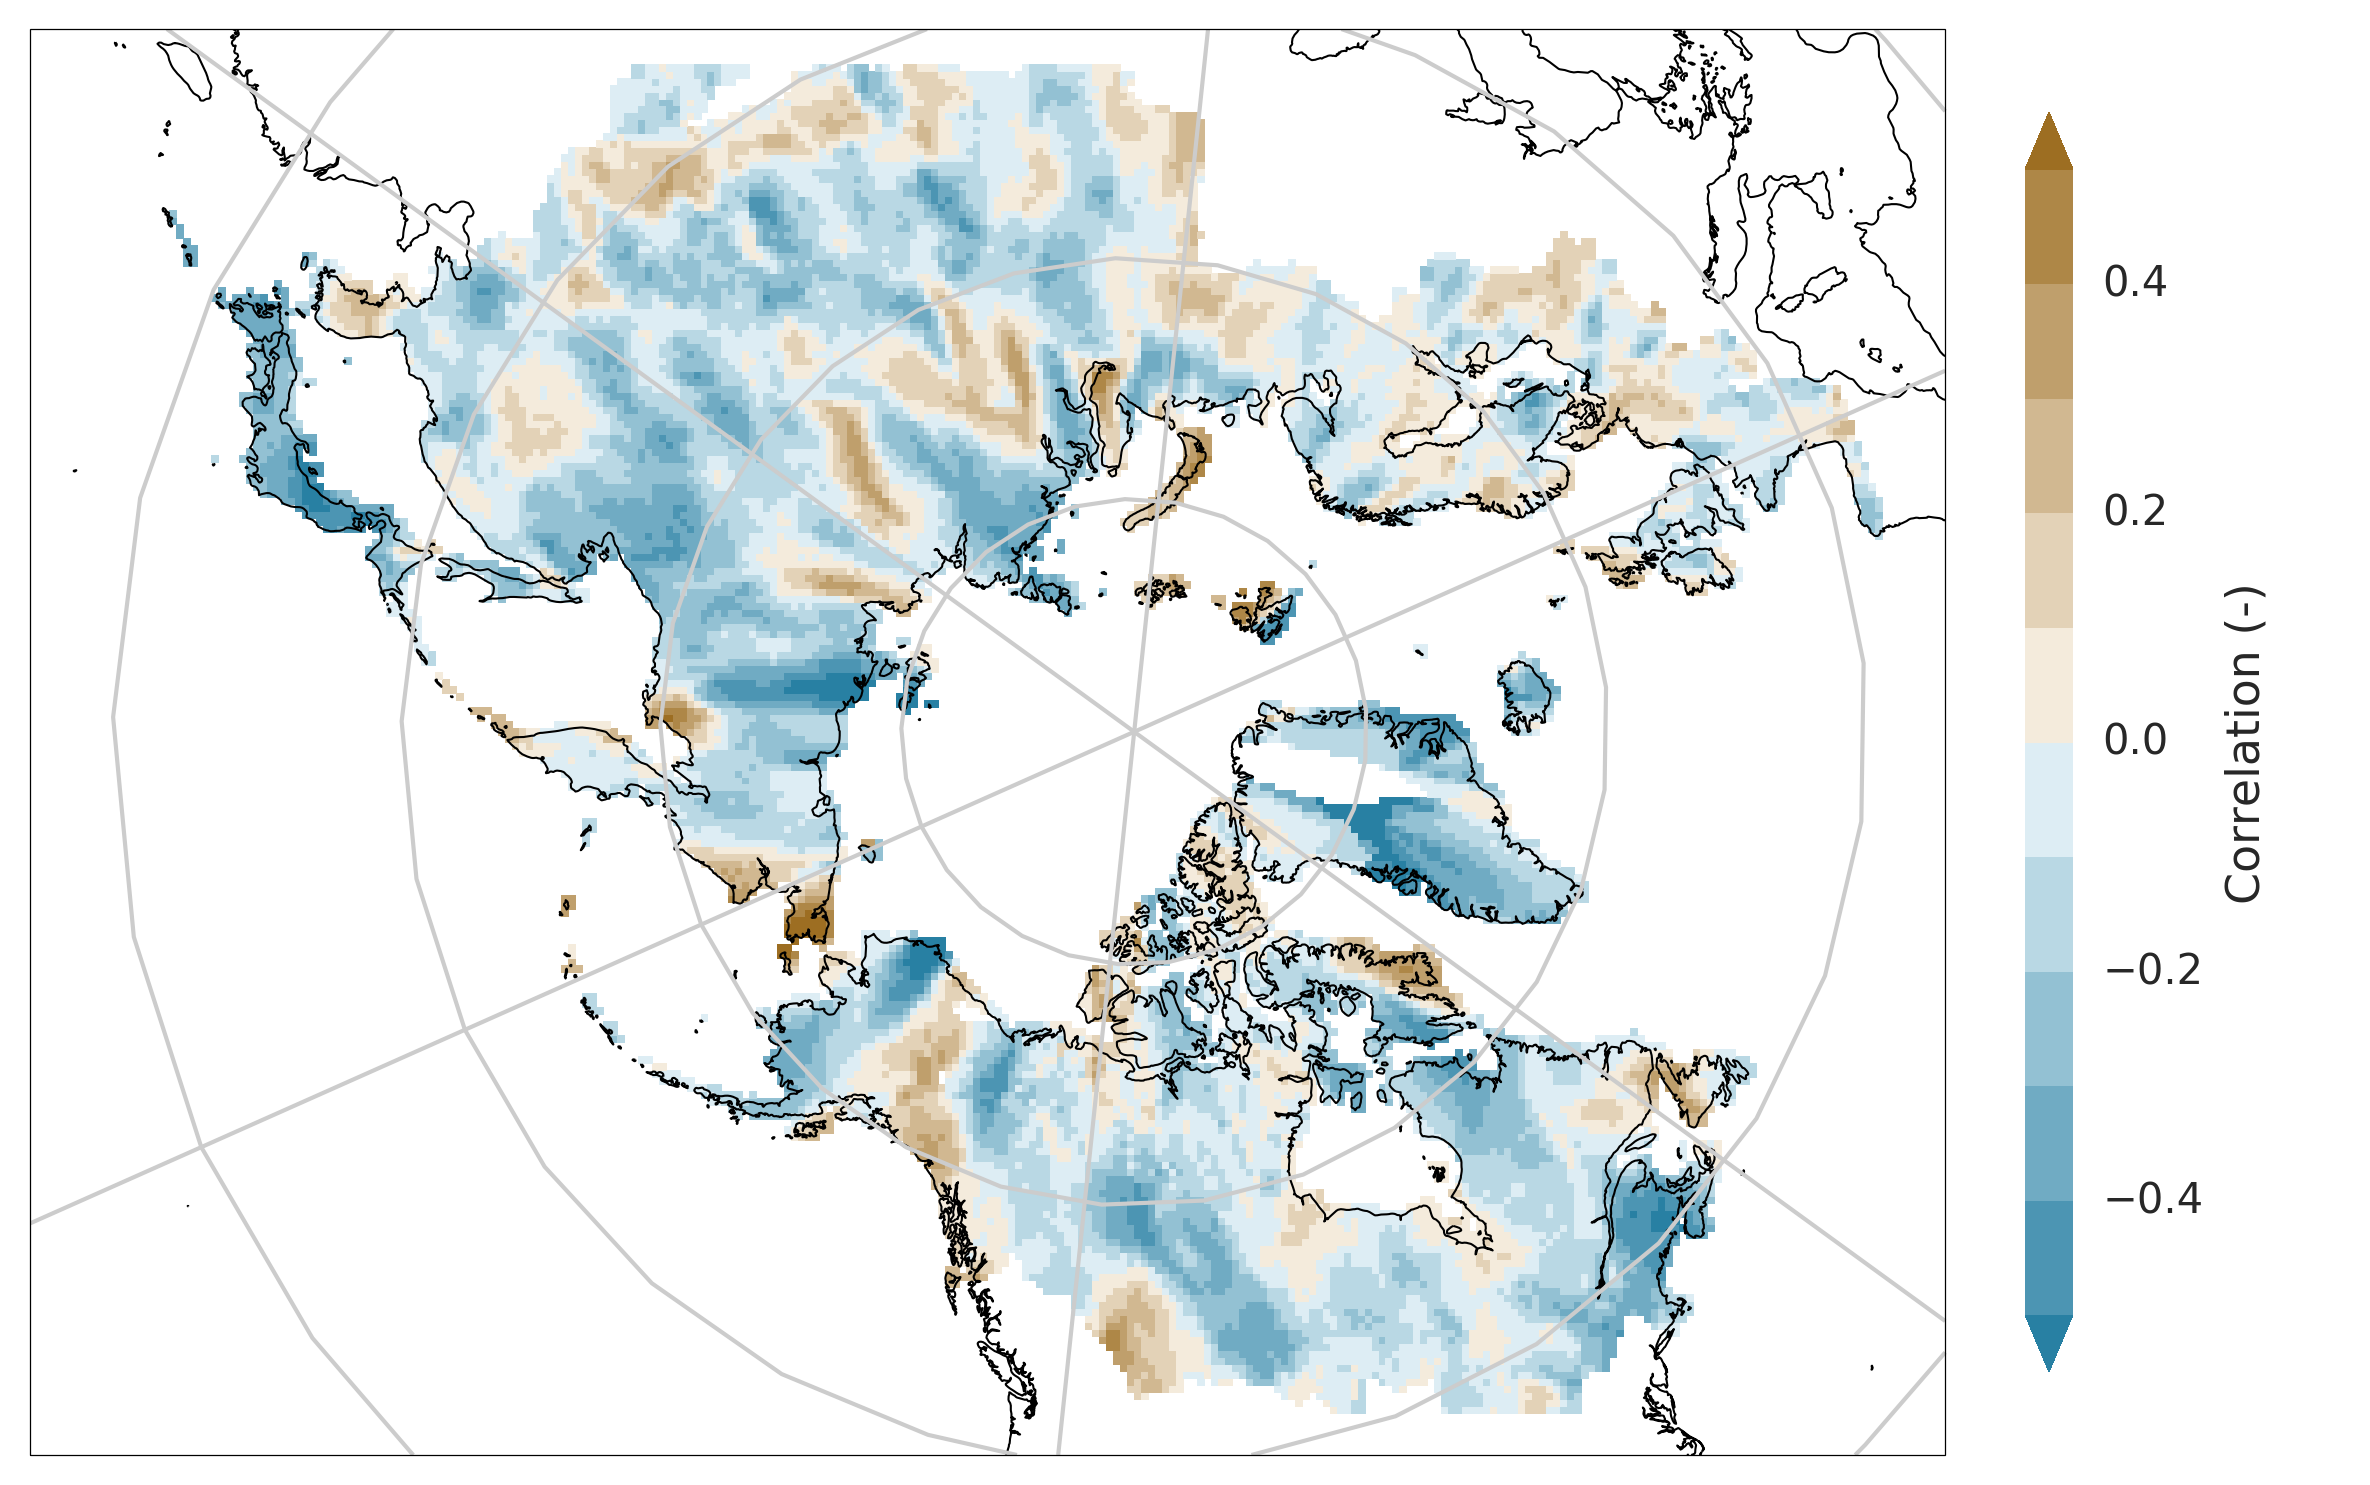
\includegraphics[width=12cm,keepaspectratio]{cru_correlation}
  \caption{Spearman rank-order correlation coefficients between observed minimum annual sea ice extent and gridded August-October precipitation from CRU. Time period 1979-2015.}
  \label{fig:prec_spatial_corr}
\end{figure}

\subsection{RASM simulations}
\label{sec:rasm_results}

% RASM sea ice sensitivity
Figure \ref{fig:sea_ice_box} shows box-and-whisker plots of sea ice extent from the three RASM simulations, described in Section \ref{sec:data_models_ch5}, compared to the NSIDC observation-based estimates.
Compared to $RASM_{CONTROL}$, $RASM_{RSI}$ and $RASM_{RSH}$ have reductions in minimum annual sea ice extents of 16\% and 49\% respectively.
In the fall, these simulations include smaller reductions in mean sea ice cover of 3\% and 11\% respectively (see also supplemental Figures \ref{fig:sea_ice_ts_sup}-\ref{fig:sea_ice_conc_sup}). % BN: I don't understand why these numbers are identical in \% from the previous version of the manuscript which looked at a different period. Are these numbers correct? Or are you referring here to the October - December period, which I would not call the fall in this context (since you already use that for August - October)
However, compared to the RASM simulations, the NSIDC observations of sea ice extent demonstrate significantly more interannual variability.
Individual months can be clearly seen in Figure \ref{fig:sea_ice_box} with the lowest values in each simulation corresponding to August (gray) and September (red) and the highest values corresponding to October (blue).
The RASM simulations have interannual standard deviations for each of these months that are 1.7 to 3.3 times smaller than the observations.
The dampened interannual variability of the individual RASM simulations is attributable to the lack a long term trend in sea ice extent (Fig. \ref{fig:sea_ice_min_ts_sup} in the supplemental material) related to a persistent radiation bias in RASM over the central Arctic in the winter \citep{Cassano_2016}.

\begin{figure}
  \centering
  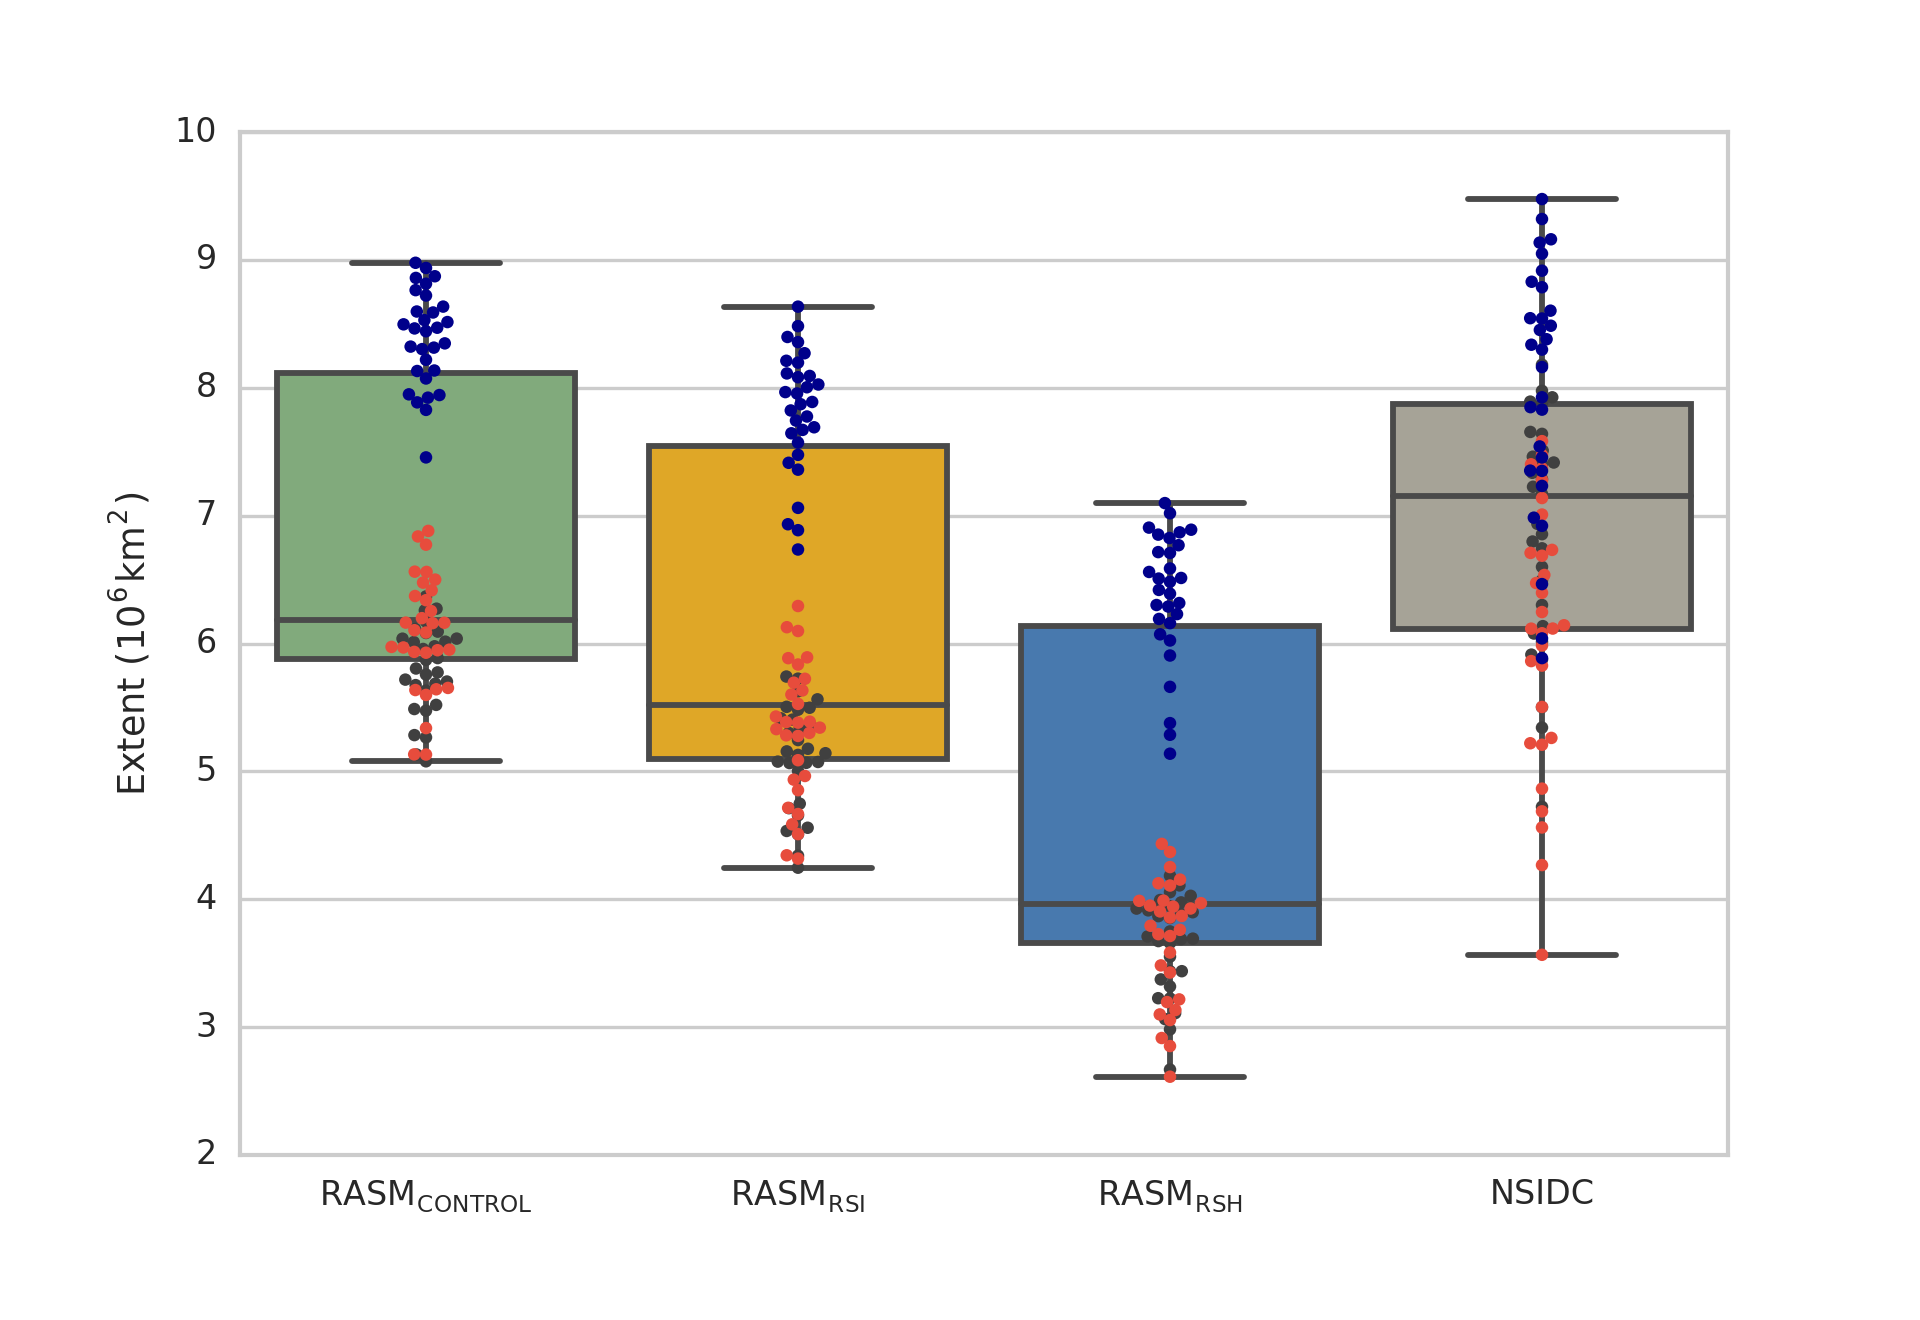
\includegraphics[width=12cm,keepaspectratio]{seaice_boxplots}
  \caption{Distribution of fall (August-October) sea ice extent in RASM and the NSIDC sea ice index. Time period 1985-2015. Each dot represents a monthly mean value for a single year for August (red), September (black) and October (blue).}
  \label{fig:sea_ice_box}
\end{figure}

Figure \ref{fig:fwb} presents the freshwater budget for the Arctic Ocean and its terrestrial drainage area, summarized for the fall months (August-October) for the three RASM simulations.
The  moisture convergence for the three simulations varies less than 27 $km^3$ per season (or 1.5\% of $RASM_{CONTROL}$), with $RASM_{RSH}$ having less moisture convergence than $RASM_{CONTROL}$.
Consequently, increases in the distribution of evaporation and precipitation shown in Figure \ref{fig:fwb} are sourced from within the central Arctic.
The reductions in sea ice extent in $RASM_{RSI}$ and $RASM_{RSH}$ are coincident with increases in ocean evaporation of 38 $km^3$ and 121 $km^3$ per season (15\% and 48\%), respectively.
These changes in evaporation from the ocean coincide with increases in precipitation over the ocean of 27 $km^3$ and 62 $km^3$ per season (3\% and 11\%) and reductions in convergence over the ocean mask of 11 $km^3$ and 60 $km^3$ (1.5\% and 8\%), respectively.
Convergence is defined here as P-E between August and October.
Finally, the precipitation over land is found to increase relative to the baseline case for both $RASM_{RSI}$ and $RASM_{RSH}$ by 26 $km^3$ and 61 $km^3$ per season (or 1\% and 2\%), respectively.
Also contributing to the increase in precipitation over land is an increase in seasonal evaporation from the land that comes in response to the reduced sea ice and associated warming of $1-3^{\circ}C$ across the high-latitude land areas.

Summarizing the water budget analysis, we find that the forced decreases in albedo in $RASM_{RSI}$ and $RASM_{RSH}$ lead to increases in divergence from the Arctic Ocean. % BN: Be careful with mixing the colloquial use of `significant` with the statistical meaning in scientific papers
Because small increases in evapotranspiration over land are balanced by small changes in convergence, the net change in precipitation over land almost entirely results from increased evaporation over the Arctic Ocean.
Changes in the spatial patterns of precipitation between the three RASM simulations (not shown) are mostly confined to the Arctic Ocean with less distinct spatial patters over land.
While this muted response may be partially explained by the limited interannual variability in the RASM sea ice extent, it also indicates that changes in evaporation from the Arctic Ocean must be accompanied with changes in circulation patterns if increases in precipitation are to be attributed to sea ice loss.

\begin{figure}
  \centering
  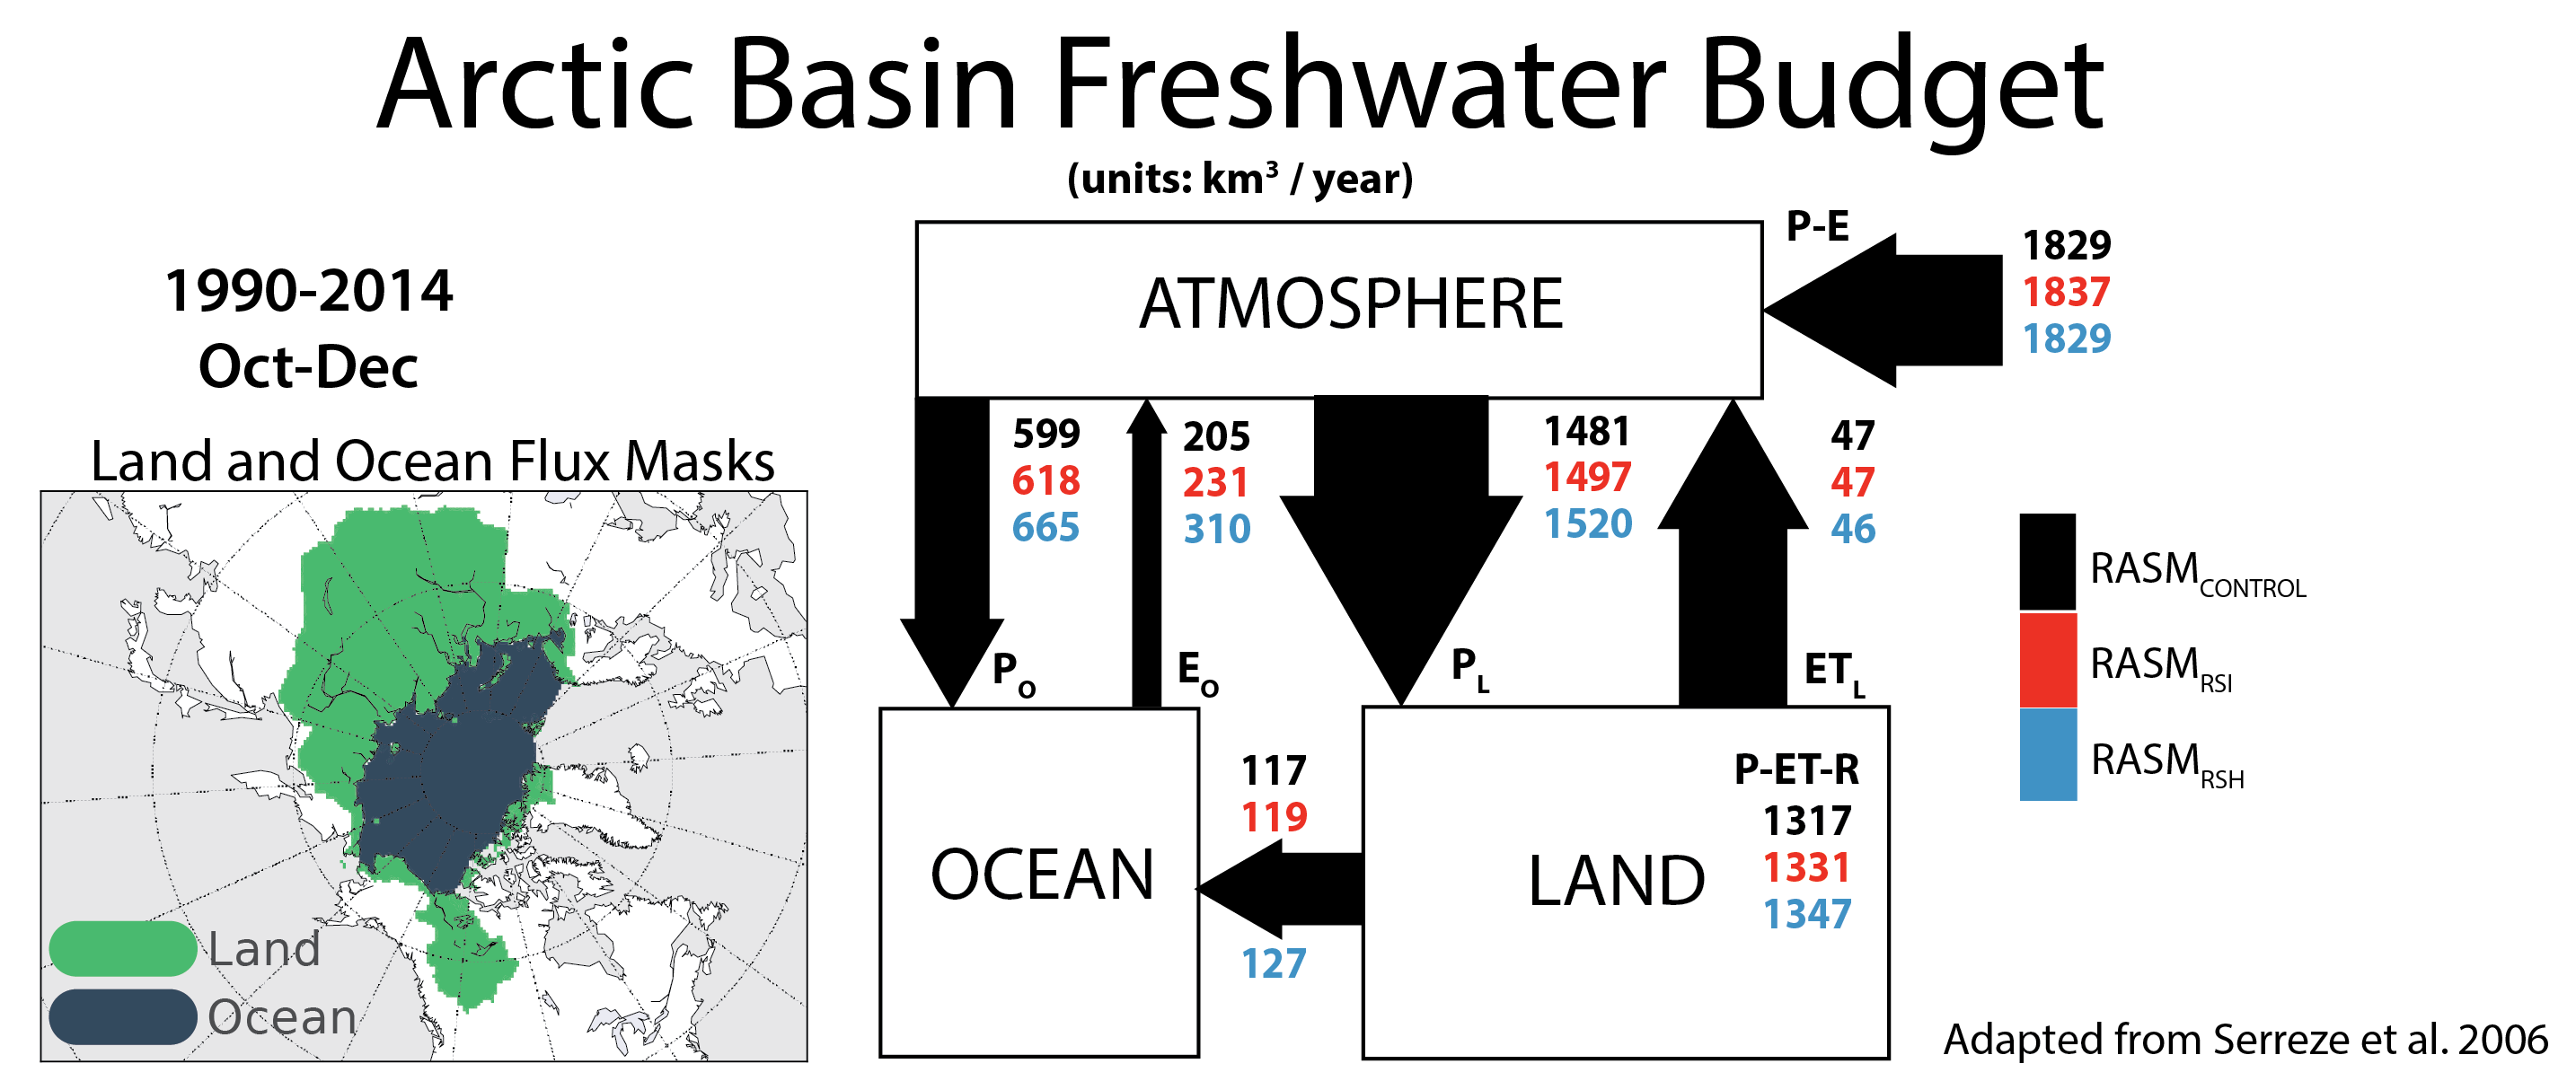
\includegraphics[width=14cm,keepaspectratio]{fresh_water_budget}
  \caption{Mean Arctic freshwater budget from RASM for the August-October period from 1985-2014 \citep[adapted from][]{Serreze_2006a}.}
  \label{fig:fwb}
\end{figure}

% SOM analysis
We have applied the SOM technique on standardized evaporation anomalies across the Arctic Ocean to better understand the coupling between ocean-sourced evaporation and anomalies in precipitation over land during the fall season.
As shown by the water budget analysis, fairly large relative increases in ocean evaporation led to small relative changes in precipitation over land, although the increases in the reduced sea ice simulations can be attributed almost entirely to increased ocean evaporation.
In applying SOMs, we will be able to connect regional patterns of ocean evaporation, sea ice extent, and atmospheric circulation to precipitation patterns over land.

% MASTER SOM
The full, trained Kohonen Layer (or Master SOM) is shown in Figure \ref{fig:master_som}.
Our analysis focuses on four SOM nodes that exhibit the largest hit rate (number of months in a particular pattern) and evaporation patterns of interest: (0,1), (1,1), (0,3), and (1,3). % BN: I do not understand the numbering. Assuming the first value is `som_x` and the second value is `som_y`, then there is no (0,3) or (1,3). If you are using `som_y, som_x`, then you need to explain that. As is, I think these should all be reversed. Alternatively change figure 5.4 to explicitly identify each SOM (as in Figure 5.6)
We will show that the first two SOMs represent generally dry patterns (low precipitation over land) while the second two represent generally wet patterns (high precipitation over land) by mapping these patterns to their coincident patterns of precipitation.
In each of these patterns, the combined position, sign, and magnitude of evaporation anomalies in the central Arctic, Kara/Barents Seas, and North Atlantic Ocean are characteristically different.

\begin{figure}
  \centering
  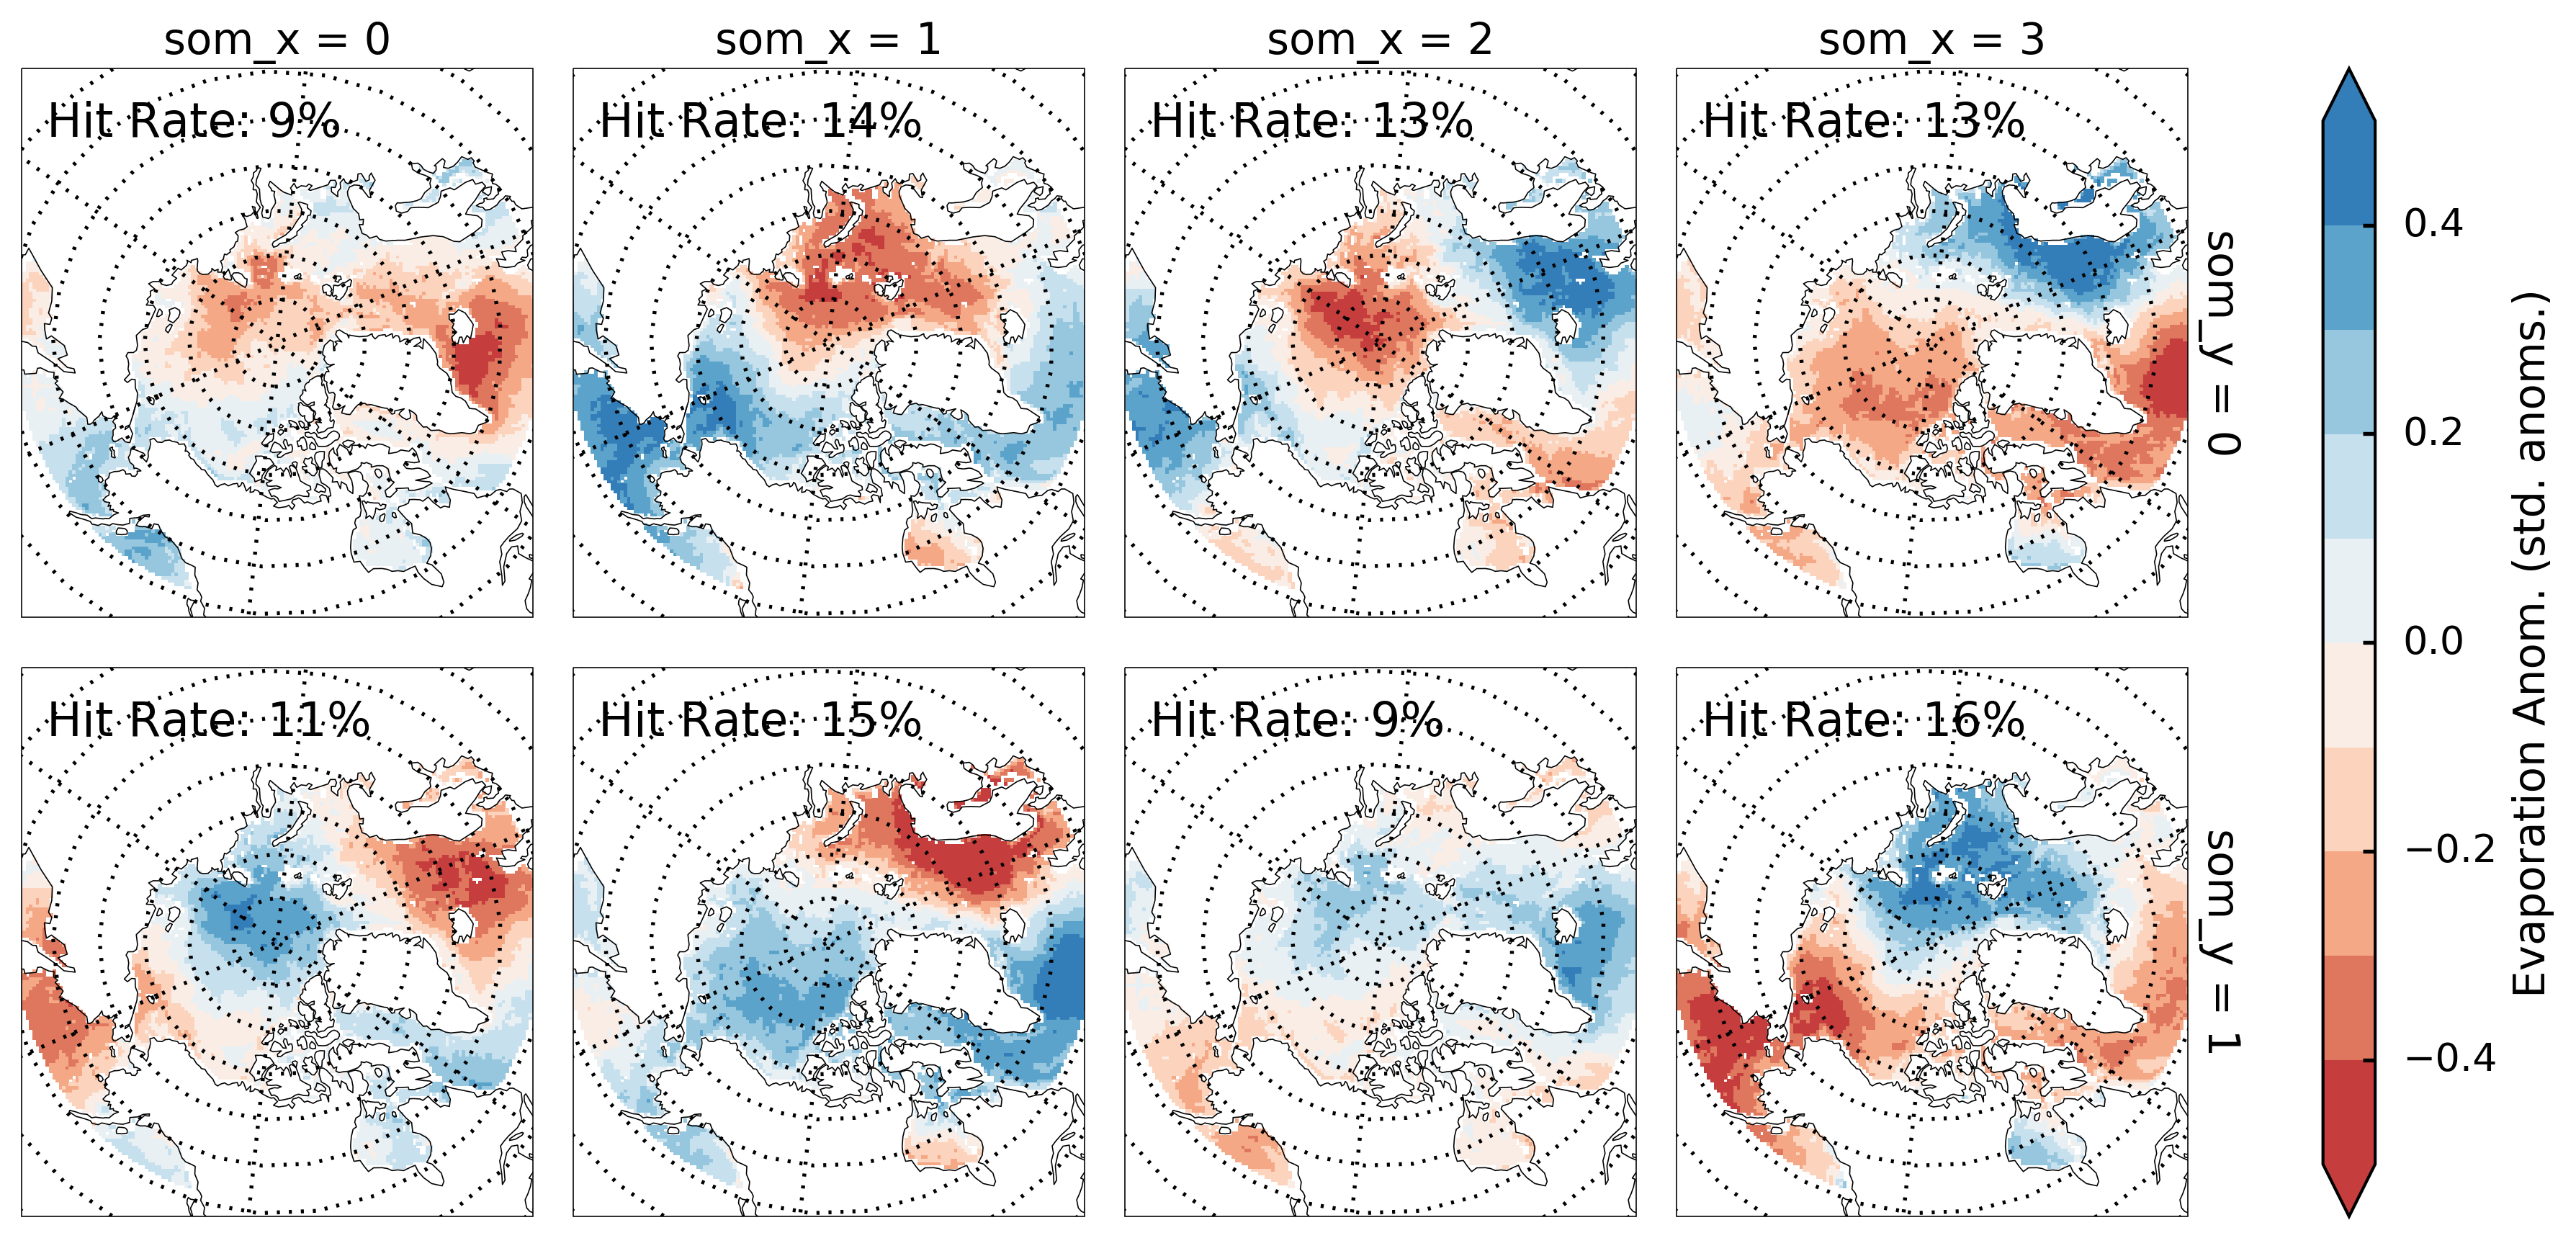
\includegraphics[width=16cm,keepaspectratio]{master_som}
  \caption{Master SOM. The hit rate, shown as the percentage of all the months (270) in the training dataset that are part of each pattern, is shown in the top left corner.} % BN: The color bar needs a label. As is, this figure is not very readable since I have no idea what is shown and how to read it. In the text you say that `spatial patterns of evaporation anomalies with patterns of positive evaporation anomalies toward the right of Figure \ref{fig:master_som} and patterns of negative evaporation anomalies toward the left.` but how am I to interpret that from this figure? I can get it from the combined SOM, but not from this figure by itself as far as I can tell. Keep in mind that most people do not use SOMs, so you need to go the extra mile to explain them. The caption should be extended to allow the figure to stand more on its own.
  % BN: Please increase the label sizes in this plot. Also since you have enought space, precede the numbers with `hit rate: X\%`
  \label{fig:master_som}
\end{figure}

% Composite SOM
Figure \ref{fig:composite_som} presents the mapped fields for the four SOM nodes discussed above.
Each of the mapped fields represents the composite mean anomalies of all months assigned to each SOM node.
Here we focus on ocean evaporation, sea level pressure (SLP), sea ice concentration, and precipitation over land.
For node (0,1), anomalously low evaporation rates from the Kara and Barents Seas are accompanied by anomalously high pressure across the Siberian Shelf.
This combination leads to negative precipitation anomalies over northern Siberia.
Node (1,1) exhibits positive evaporation anomalies in the central Arctic and negative evaporation anomalies in the Kara and Barents Seas.
SLPs for this node are anomalously low over Greenland and high over Northern Europe.
Corresponding precipitation anomalies for node (1,1) are negative over Northern Europe and near normal across Siberia.
Interestingly, this SOM node shows the strongest pattern of negative sea ice anomalies, located near the eastern Siberian Shelf.
However, adjacent land regions only show relatively small positive anomalies over Siberia and negative anomalies over Alaska.

\begin{figure}
  \centering
  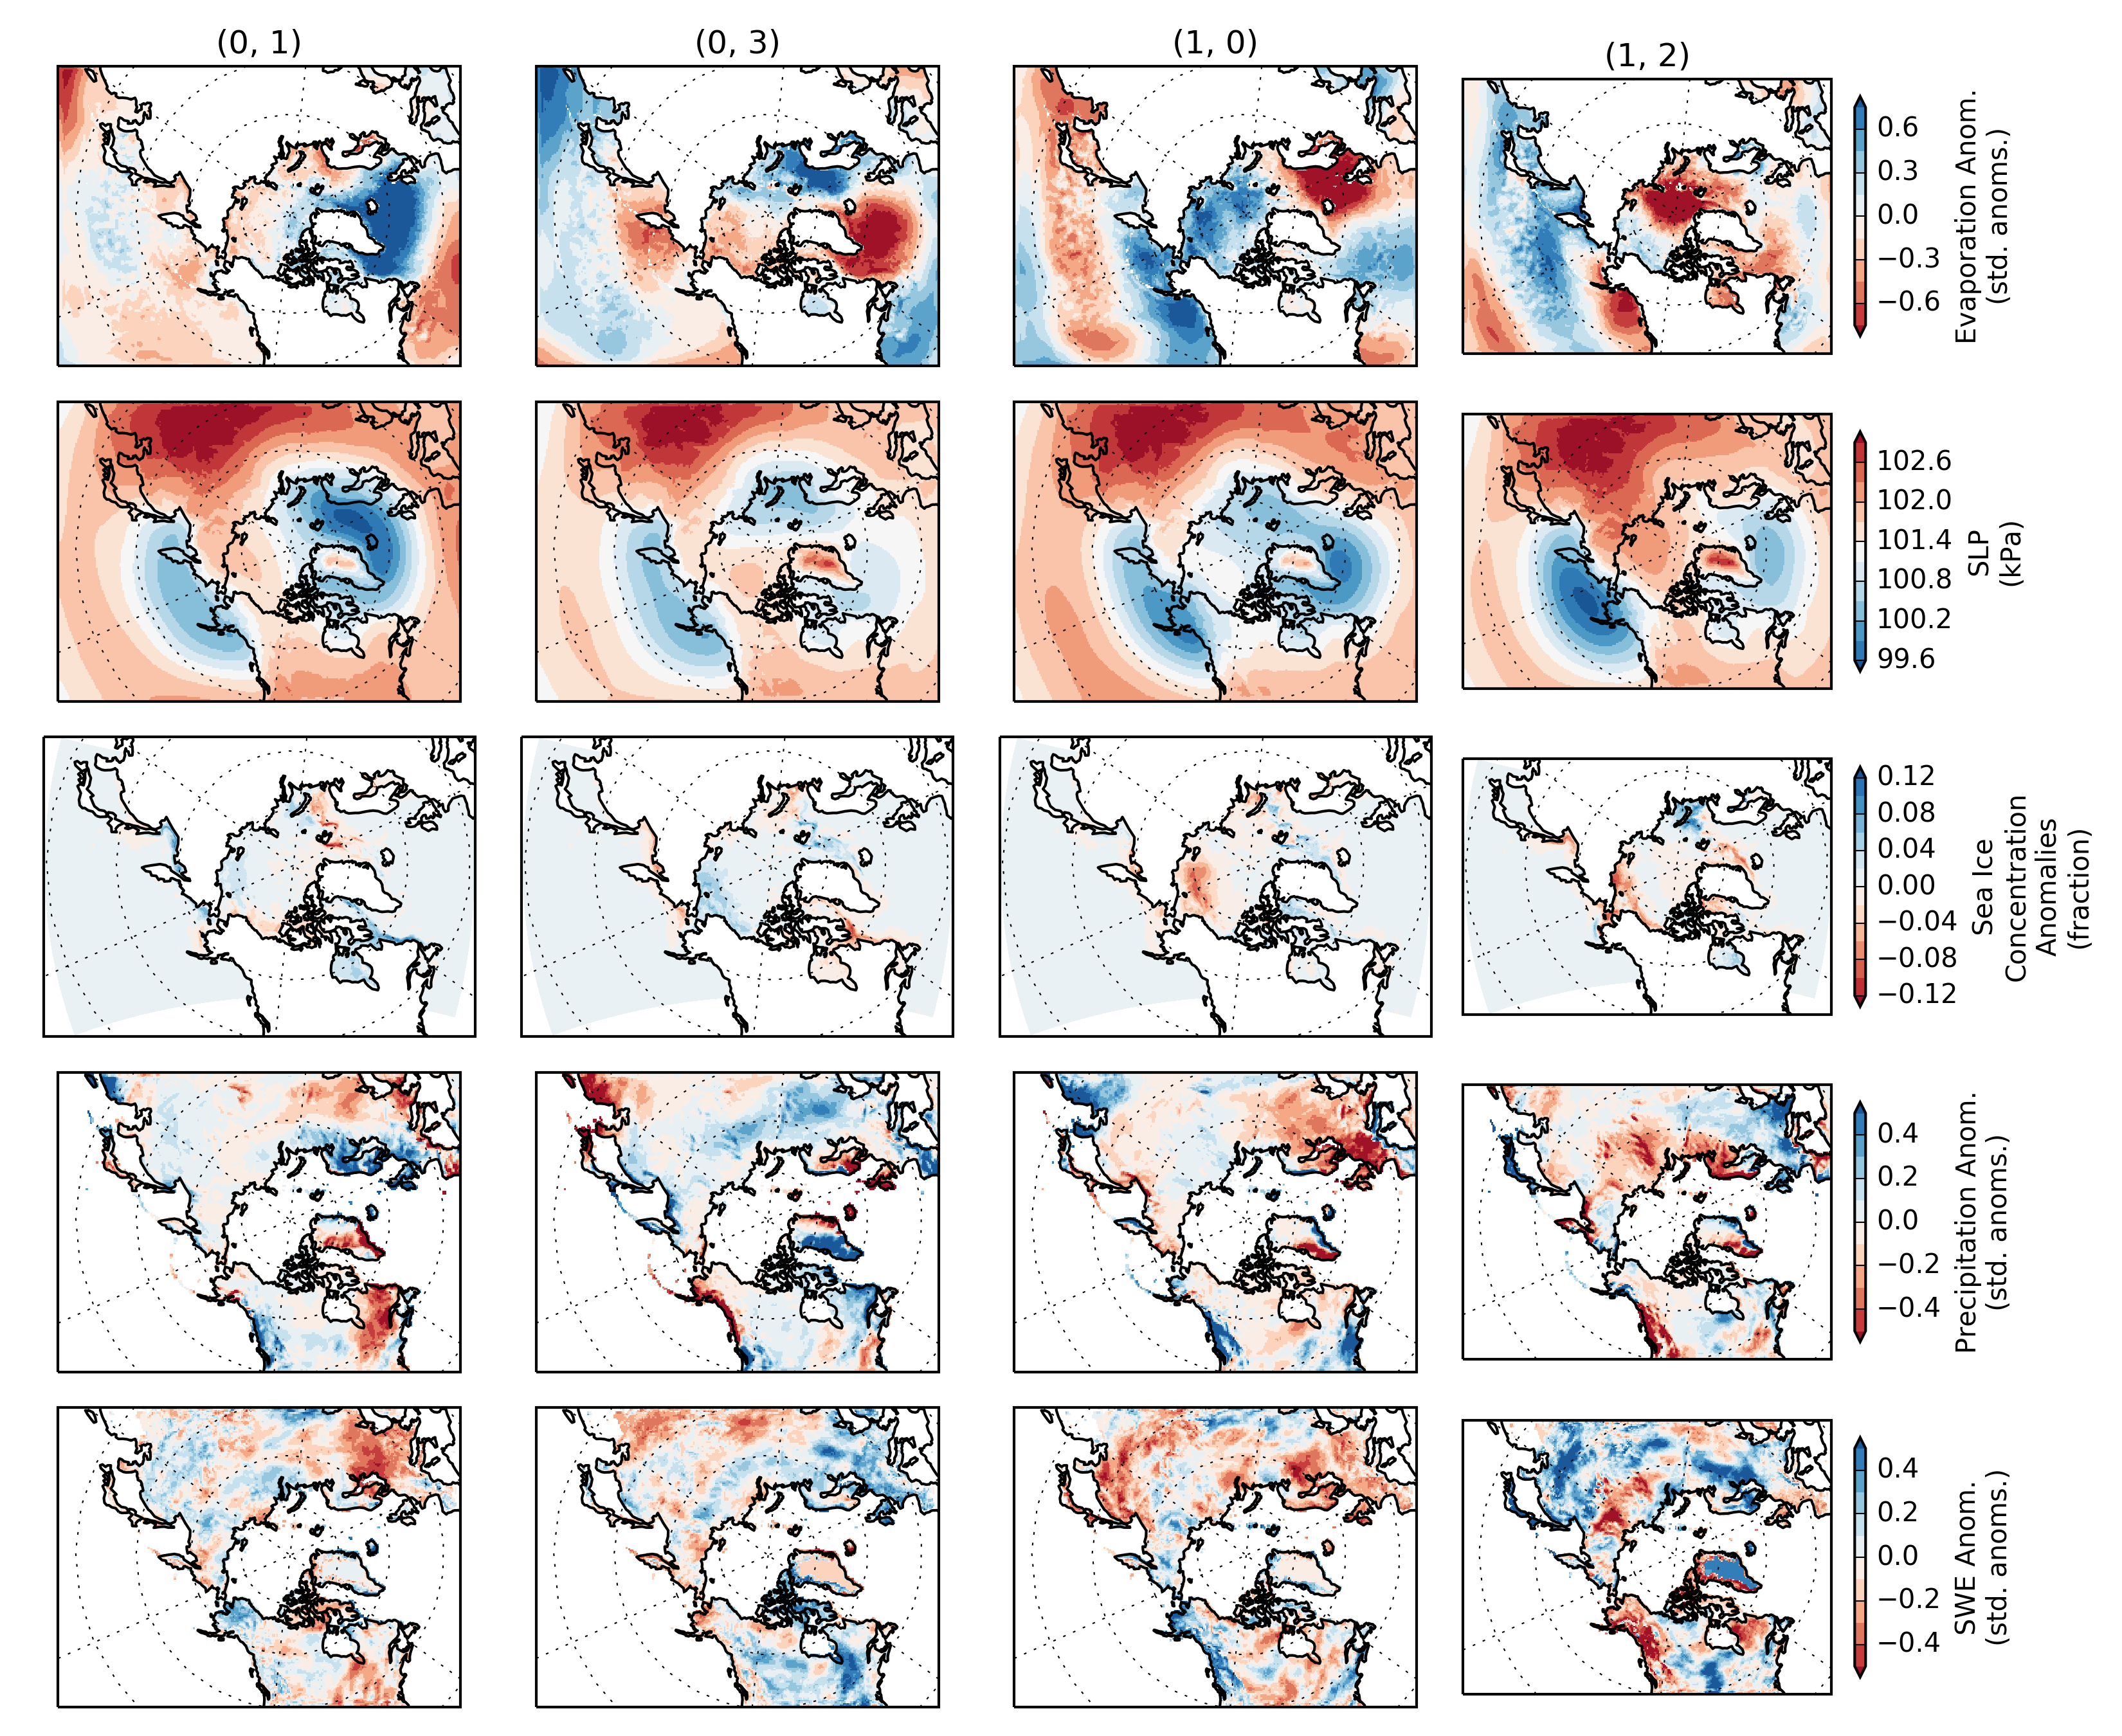
\includegraphics[width=16cm,keepaspectratio]{composite_som}
  \caption{SOM nodes (0,1), (1,1), (0,3), and (1,3) mapped to ocean evaporation, sea level pressure (SLP), sea ice concentration, and precipitation over land. Values plotted are the average anomalies across all the members of each node.} % BN : See comment above about numbering
  % BN : May improve readability to repeat the SOM in the first row
  \label{fig:composite_som}
\end{figure}

Node (0,3) exhibits positive evaporation anomalies across the European side of the Arctic Ocean, accompanied by lower than normal pressures over Northern Europe. % BN: Please do NOT use the `positive (negative)` notation as it is confusing and ugly. There is a good post or article from Alan Robock somewhere bitching about this and I fully agree.
Node (1,3) shows positive ocean evaporation anomalies near Siberia and lower than normal pressures over Northern Siberia (1,3).
These patterns lead to positive anomalies in precipitation over land, particularly when the SLP patterns would encourage onshore flow from regions with positive anomalies in evaporation.
The lack of strong correspondence between sea ice and evaporation anomalies indicates that variability in the fall evaporation flux in RASM is largely being driven by patterns in the ocean and atmosphere rather than changes in sea ice.

% Hit Map
The trained SOM can be used to identify the frequency of occurrence of each pattern as a function of month (August, September, or October) and RASM simulation ($RASM_{CONTROL}$, $RASM_{RSI}$, or $RASM_{RSH}$).
Figure \ref{fig:som_hit_freq} plots the pattern frequency, by month and simulation, for each node in the 2x4 SOM.
Nodes (0,1) and (1,1), which have a large region of positive evaporation anomalies across the Kara and Barents Seas, occur less frequently in $RASM_{RSH}$ as in $RASM_{CONTROL}$.
The opposite is found in node (1,3), where the pattern frequency is found to increase under reduced sea ice conditions.
On the whole, the SOM analysis indicates that decreasing sea ice extent and the associated evaporation changes are most likely to contribute to wetting trends over land when these changes are accompanied by a shift in atmospheric circulation (e.g. node (1,3)).
Global climate models tend to suggest that future Arctic climate will be stormier \citep{Vavrus_2012} and that fall and winter circulation patters may trend toward a more variable pattern.
However, the patterns with large shifts in frequency ([)nodes (0,1) and (1,1)) change in ways that limit the impact of sea ice loss, which indicates that the precipitation response may be dampened.

\begin{figure}
  \centering
  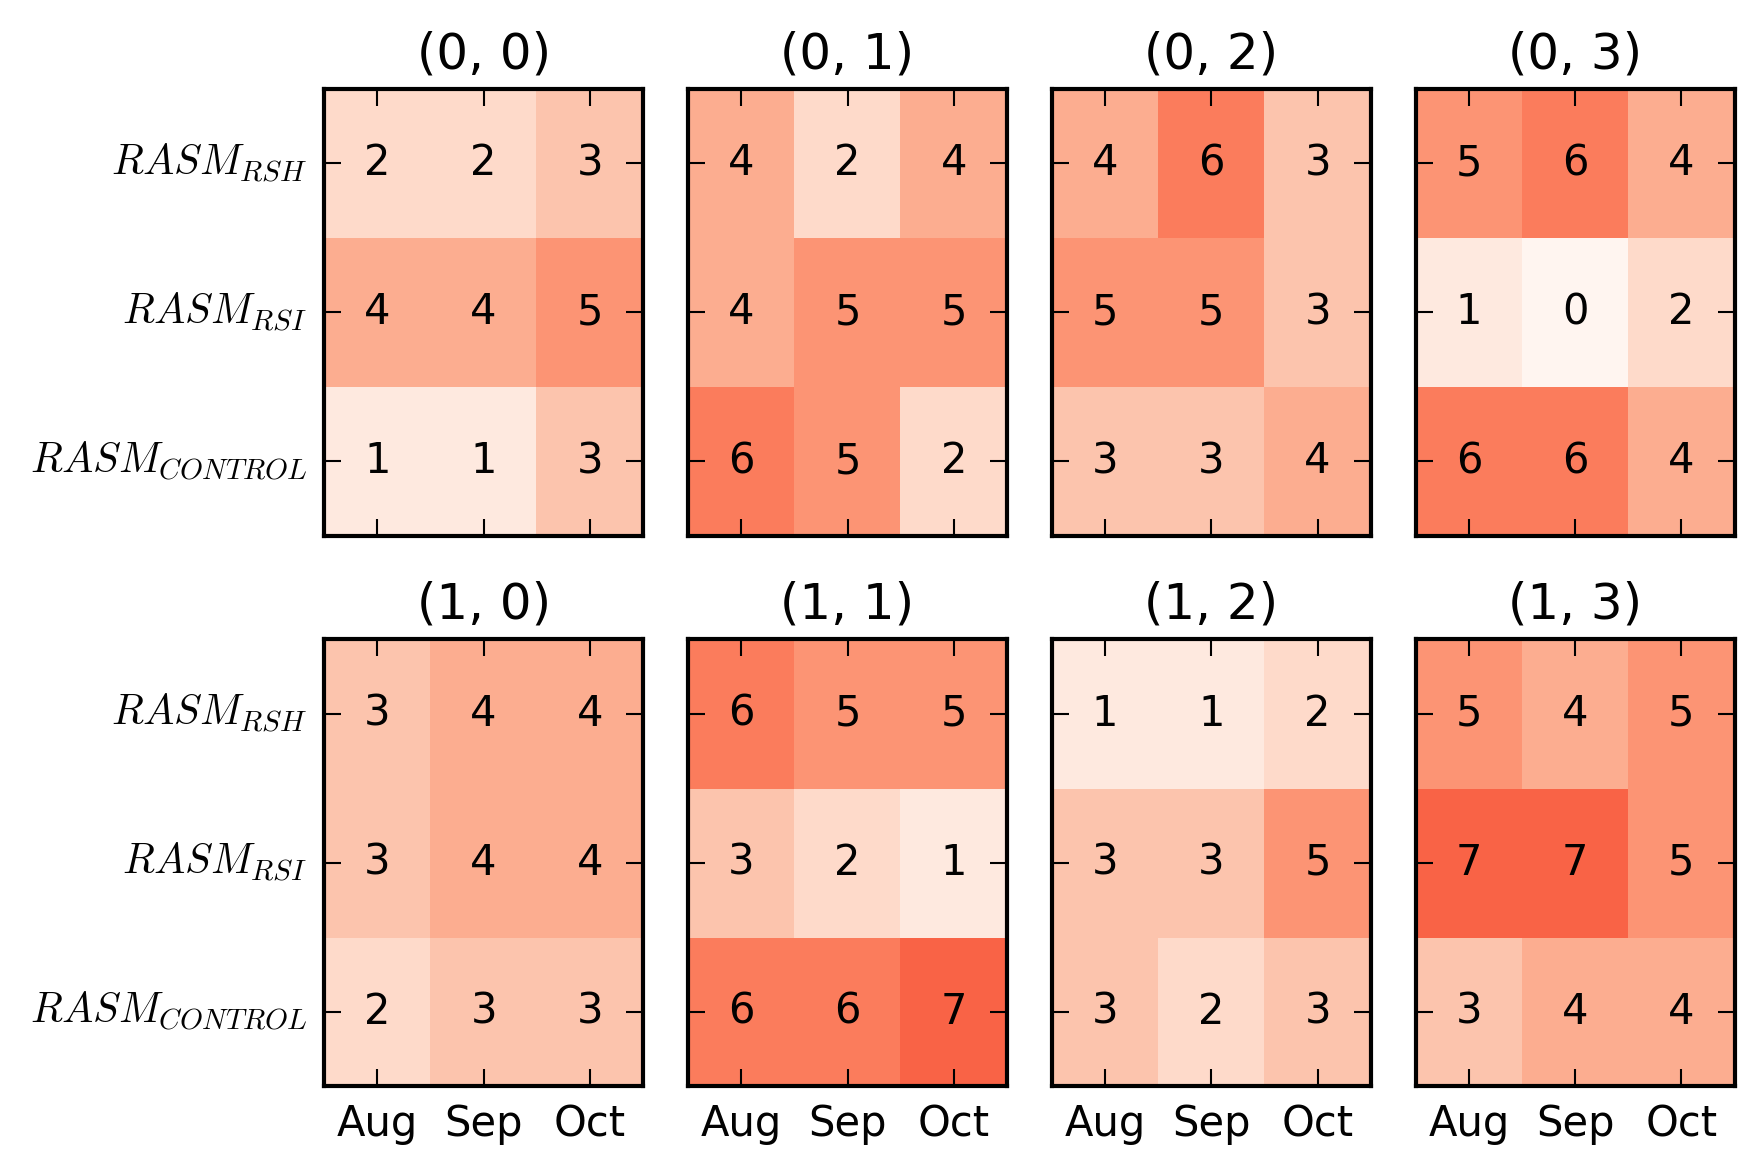
\includegraphics[width=12cm,keepaspectratio]{som_hit_freq}
  \caption{SOM pattern frequency by month and RASM simulation.} % BN: Caption needs to be expanded. What do the colors mean? Figure often end iup leading a life of their own and should be more self-containted.
  % BN: Why are you showing all the SOMS here rather than only the four that you selected for analysis

  \label{fig:som_hit_freq}
\end{figure}

\section{Conclusions}
\label{sec:conclusions_ch5}
We have investigated the relationship between sea ice extent and fall precipitation over the Pan Arctic land areas.
We have demonstrated an interannual covariation between observations of sea ice extent and precipitation over land.
Our initial hypothesis was that variations in sea ice extent were a driving factor in precipitation over land in the fall.
A water budget analysis highlighted that relatively large changes in fall evaporation from the Arctic Ocean are expected (\~50\% in our simulation with the lowest sea ice concentration), but that these changes lead to only relatively small changes in the precipitation flux over land.
However, our analysis also attributed almost all of the increases in precipitation to increases in ocean evaporation.
Furthermore, the modest increases in terrestrial fall season precipitation simulated by RASM under reduced sea ice conditions indicate that there will have to be significant circulation changes in the future if ocean sourced evaporation is to significantly impact precipitation over land.
Our SOM analysis has also pointed us in this direction, which is that the ties between evaporation and precipitation are only robust under certain atmospheric circulations.
Across Eurasia, the dominant coupling between precipitation and Arctic Ocean evaporation requires low pressure anomalies over the central Arctic, similar to the negative phase of the Arctic Oscillation \citep{Thompson_1998}.
Previous work by \citet{Cassano_2014}, using partially coupled global simulations with prescribed sea ice, has also indicated that reductions in sea ice extent in the fall may contribute to negative sea level pressure anomalies over the Arctic Ocean.

Of particular interest is the sea ice state of the Kara and Barents Seas.
As sea ice declines, we expect that this coupling will become stronger, especially if the Arctic is to become stormier.
We have found that sea ice retreat along the Siberian shelf and north Alaskan coast exerts less influence on precipitation regional patterns.
In these areas, the circulation patterns related to the Aleutian Low (low pressure in North Pacific) tend to limit the influence of enhanced evaporation along the retreating ice edge.
